\documentclass{article}

\usepackage{titlesec}

\usepackage{amsmath}
\usepackage{amssymb}

\usepackage{booktabs}
\usepackage{float}
\usepackage{colortbl}
\usepackage{xcolor}

\usepackage{a4wide}
\usepackage{setspace}
\usepackage{geometry}
\usepackage{parskip}

\usepackage{multirow}
\usepackage{adjustbox}
\usepackage{graphicx}

\usepackage{listings}
\lstdefinestyle{mystyle}{
    basicstyle=\ttfamily
}

\lstset{style=mystyle
}

\renewcommand{\familydefault}{\sfdefault}

\usepackage{hyperref}
\hypersetup{
    colorlinks=true,
    linkcolor=black,
    urlcolor=blue
}

\DeclareRobustCommand{\bbone}{\text{\usefont{U}{bbold}{m}{n}1}}

\titleformat*{\subsubsection}{\normalfont}

\author{Yu Xia \\ ID: yx5262}
\title{\textbf{Yu Xia's A4}}
\date{October 2022}

\begin{document}
\maketitle

\nocite{*}

\section*{\textrm{Multiple Choice}}

1-5:\\
abccc

6-10:\\
bacdc

11-15:\\
adada

\section*{\textrm{Long}}

\subsection*{\textrm{1. Optimal monetary policy, flexible price model}}

\subsubsection*{\textrm{a.}}

\fbox{%
\parbox[c]{\textwidth}{\
\begin{equation*}
    \begin{aligned}
    & \max\sum_{s=0}^{\infty}\beta^{s}U\left(c_{t+s},1-n_{t+s}\right) \\
     \textrm{subject to}\\
    & W_{t}n_{t}+\left(S_{t}+D_{t}\right)a_{t-1}+B_{t-1}+M_{t-1}+\tau_{t}=P_{t}c_{t}+S_{t}a_{t}+P^{b}_{t}B_{t}+M_{t}, \\
    & \left(S_{t}+D_{t}\right)a_{t-1}+B_{t-1}+M_{t-1}+\tau_{t}=P_{t}c_{t}+S_{t}a_{t}+P^{b}_{t}B_{t}.
    \end{aligned}
\end{equation*}%
}}

\subsubsection*{\textrm{b.}}

Stage 1:

Financial market opens, consumers trade in the market, and the financial market closes.

Step 2:

Consumers use what they left (in terms of income) to buy goods.

Step 3:

Consumers get their wage income.

\subsubsection*{\textrm{c.}}

The Lagrangian is
\begin{flalign*}
    \mathcal{L} & = \sum_{s=0}^{\infty}\beta^{s}U\left(c_{t+s},1-n_{t+s}\right) \\
    &-\lambda_{t}\left(W_{t}n_{t}+\left(S_{t}+D_{t}\right)a_{t-1}+B_{t-1}+M_{t-1}+\tau_{t}-P_{t}c_{t}-S_{t}a_{t}-P^{b}_{t}B_{t}-M_{t}\right) \\
    &-\mu_{t}\left(\left(S_{t}+D_{t}\right)a_{t-1}+B_{t-1}+M_{t-1}+\tau_{t}-P_{t}c_{t}-S_{t}a_{t}-P^{b}_{t}B_{t}\right)\\
    &-\beta\lambda_{t+1}\left(W_{t+1}n_{t+1}+\left(S_{t+1}+D_{t+1}\right)a_{t}+B_{t}+M_{t}+\tau_{t+1}-P_{t+1}c_{t+1}-S_{t+1}a_{t+1}-P^{b}_{t+1}B_{t+1}-M_{t+1}\right)\\
    &-\beta\mu_{t+1}\left(\left(S_{t+1}+D_{t+1}\right)a_{t}+B_{t}+M_{t}+\tau_{t+1}-P_{t+1}c_{t+1}-S_{t+1}a_{t+1}-P^{b}_{t+1}B_{t+1}\right)\\
    &+\dots
\end{flalign*}

FOC w.r.t. $c_{t}$:

$U_{c}-\lambda_{t}\left(-P_{t}\right)-\mu_{t}\left(-P_{t}\right)=0$

$\iff$

$U_{c}+\lambda_{t}P_{t}+\mu_{t}P_{t}=0$

$\iff$
\begin{flalign}
    \dfrac{U_{c}}{P_{t}} &=-\lambda_{t}-\mu_{t}&
\end{flalign}
%(1)

FOC w.r.t. $n_{t}$:

$U_{l}\cdot\left(-1\right)-\lambda_{t}W_{t}=0$

$\iff$

$U_{l}=-\lambda_{t}W_{t}$

$\iff$
\begin{flalign}
    \dfrac{U_{l}}{W_{t}}&=-\lambda_{t}&
\end{flalign}
%(2)
FOC w.r.t. $a_{t}$:

$-\lambda_{t}\left(-S_{t}\right)-\mu_{t}\left(-S_{t}\right)-\beta\lambda_{t+1}\left(S_{t+1}+D_{t+1}\right)-\beta\mu_{t+1}\left(S_{t+1}+D_{t+1}\right)=0$

$\iff$

$\lambda_{t}S_{t}+\mu_{t}S_{t}-\beta\lambda_{t+1}\left(S_{t+1}+D_{t+1}\right)-\beta\mu_{t+1}\left(S_{t+1}+D_{t+1}\right)=0$

$\iff$

$\left(\lambda_{t}+\mu_{t}\right)S_{t}-\beta\left(\lambda_{t+1}+\mu_{t+1}\right)\left(S_{t+1}+D_{t+1}\right)=0$

$\iff$

$\left(\lambda_{t}+\mu_{t}\right)S_{t}=\beta\left(\lambda_{t+1}+\mu_{t+1}\right)\left(S_{t+1}+D_{t+1}\right)$

$\iff$
\begin{flalign}
    S_{t}&=\dfrac{\beta\left(\lambda_{t+1}+\mu_{t+1}\right)\left(S_{t+1}+D_{t+1}\right)}{\lambda_{t}+\mu_{t}}&
\end{flalign}
%(3)
FOC w.r.t. $B_{t}$:

$-\lambda_{t}\left(-P^{b}_{t}\right)-\mu_{t}\left(-P^{b}_{t}\right)-\beta\lambda_{t+1}-\beta\mu_{t+1}=0$

$\iff$

$\lambda_{t}P^{b}_{t}+\mu_{t}P^{b}_{t}-\beta\lambda_{t+1}-\beta\mu_{t+1}=0$

$\iff$

$\left(\lambda_{t}+\mu_{t}\right)P^{b}_{t}=\beta\lambda_{t+1}+\beta\mu_{t+1}$

$\iff$
\begin{flalign}
    P^{b}_{t}&=\dfrac{\beta\left(\lambda_{t+1}+\mu_{t+1}\right)}{\lambda_{t}+\mu_{t}}&
\end{flalign}
%(4)
FOC w.r.t. $M_{t}$:

$-\lambda_{t}\cdot\left(-1\right)-\beta\lambda_{t+1}-\beta\mu_{t+1}=0$

$\iff$
\begin{flalign}
    \lambda_{t}&=\beta\left(\lambda_{t+1}+\mu_{t+1}\right)&
\end{flalign}
%(5)
\subsubsection*{\textrm{d.}}

Plug (5) into (4), we have:

$P^{b}_{t}=\dfrac{\lambda_{t}}{\lambda_{t}+\mu_{t}}$

$\iff$

$\dfrac{\lambda_{t}+\mu_{t}}{\lambda_{t}}=\dfrac{1}{P^{b}_{t}}$

$\iff$

$\lambda_{t}+\mu_{t}=\dfrac{\lambda_{t}}{P^{b}_{t}}$

$\iff$

$\mu_{t}=\lambda_{t}\left(\dfrac{1}{P^{b}_{t}}-1\right)=\lambda_{t}\dfrac{1-P^{b}_{t}}{P^{b}_{t}}$

$\because 1+i_{t}=\dfrac{1}{P^{b}_{t}}$

\begin{flalign}
    \mu_{t}&=i_{t}\lambda_{t}&
\end{flalign}
%(6)

By (1) and (2), we have:

$\dfrac{U_{c}}{U_{l}}=\dfrac{P_{t}\left(-\lambda_{t}-\mu_{t}\right)}{-\lambda_{t}W_{t}}=\dfrac{P_{t}\left(\lambda_{t}+\mu_{t}\right)}{\lambda_{t}W_{t}}$

$\dfrac{U_{l}}{U_{c}}=\dfrac{W_{t}}{P_{t}}\cdot\dfrac{\lambda_{t}}{\lambda_{t}+\mu_{t}}=\dfrac{1}{1+\dfrac{\mu_{t}}{\lambda_{t}}}\cdot w_{t}$

Therefore,
\begin{flalign}
    \dfrac{U_{l}\left(c_{t},1-n_{t}\right)}{U_{c}\left(c_{t},1-n_{t}\right)}&=\dfrac{w_{t}}{1+i_{t}}&
\end{flalign}
%(7)

If $i_{t}=0$, it is the same with the previous model we've learned. The $MRS$ between labor and consumption is the real wage. 

If $i_{t}>0$, however, there is a wedge between $MRS$ and the real wage. Because consumers have to satisfy the CIA constraint, they spend their wage in the next period. Consumers hold cash and give up the benefit coming from the interest rate. So the higher $i$ is, the less consumers will gain from working, compared to the financial market. 

By (1), we have:
\begin{flalign*}
    \dfrac{\lambda_{t+1}+\mu_{t+1}}{\lambda_{t}+\mu_{t}} &=\dfrac{-\lambda_{t+1}-\mu_{t+1}}{-\lambda_{t}-\mu_{t}}&\\
    &=\dfrac{\dfrac{U_{c}\left(c_{t+1},1-n_{t+1}\right)}{P_{t+1}}}{\dfrac{U_{c}\left(c_{t},1-n_{t}\right)}{P_{t}}}&\\
    &=\dfrac{U_{c}\left(c_{t+1},1-n_{t+1}\right)}{U_{c}\left(c_{t},1-n_{t}\right)}\cdot\dfrac{P_{t}}{P_{t+1}}&\\
    &=\dfrac{U_{c}\left(c_{t+1},1-n_{t+1}\right)}{U_{c}\left(c_{t},1-n_{t}\right)}\cdot\dfrac{1}{\dfrac{P_{t+1}}{P_{t}}}&\\
    &=\dfrac{U_{c}\left(c_{t+1},1-n_{t+1}\right)}{U_{c}\left(c_{t},1-n_{t}\right)}\cdot\dfrac{1}{1+\pi_{t+1}}
\end{flalign*}

Plug in equation (4):

$P^{b}_{t}\dfrac{U_{c}\left(c_{t},1-n_{t}\right)}{U_{c}\left(c_{t+1},1-n_{t+1}\right)}=\beta\dfrac{1}{1+\pi_{t+1}}$

By Fisher Equation:
\begin{flalign}
    1+i_{t}&=\left(1+\pi_{t+1}\right)\left(1+r_{t}\right)&
\end{flalign}
%(8)

$\iff$

$\dfrac{1+i_{t}}{1+\pi_{t+1}}=1+r_{t}$

$\iff$

$\dfrac{1}{1+\pi_{t+1}}=\dfrac{1}{1+i_{t}}\left(1+r_{t}\right)=P^{b}_{t}\left(1+r_{t}\right)$

Hence
\begin{flalign}
    \dfrac{U_{c}\left(c_{t},1-n_{t}\right)}{U_{c}\left(c_{t+1},1-n_{t+1}\right)}&=\beta\left(1+r_{t}\right)&
\end{flalign}
%(9)

The intertemporal $MRS$ provides us with the intuition that the opportunity cost of consuming today and tomorrow is related to how impatient consumers are ($\beta$), and the real interest rate.

$\because\dfrac{U_{l}\left(c_{t},1-n_{t}\right)}{U_{c}\left(c_{t},1-n_{t}\right)}=\dfrac{w_{i}}{1+i_{t}}$

$\therefore U_{l}\left(c_{t},1-n_{t}\right)=\dfrac{w_{t}}{1+i_{t}}U_{c}\left(c_{t},1-n_{t}\right)$

$U_{l}\left(c_{t+1},1-n_{t+1}\right)=\dfrac{w_{t+1}}{1+i_{t+1}}U_{c}\left(c_{t+1},1-n_{t+1}\right)$

$\therefore\dfrac{U_{l}\left(c_{t},1-n_{t}\right)}{U_{l}\left(c_{t+1},1-n_{t+1}\right)}=\dfrac{\dfrac{w_{t}}{1+i_{t}}U_{c}\left(c_{t},1-n_{t}\right)}{\dfrac{w_{t+1}}{1+i_{t+1}}U_{c}\left(c_{t+1},1-n_{t+1}\right)}=\dfrac{\dfrac{w_{t}}{1+i_{t}}}{\dfrac{w_{t+1}}{1+i_{t+1}}}\cdot\dfrac{U_{c}\left(c_{t},1-n_{t}\right)}{U_{c}\left(c_{t+1},1-n_{t+1}\right)}$

$\because\dfrac{U_{c}\left(c_{t},1-n_{t}\right)}{U_{c}\left(c_{t+1},1-n_{t+1}\right)}=\beta\left(1+r_{t}\right)$

$\therefore\dfrac{U_{l}\left(c_{t},1-n_{t}\right)}{U_{l}\left(c_{t+1},1-n_{t+1}\right)}=\dfrac{\dfrac{w_{t}}{1+i_{t}}}{\dfrac{w_{t+1}}{1+i_{t+1}}}\cdot\beta\left(1+r_{t}\right)$

If $i_{t+1}=i_{t}$,

$\dfrac{U_{l}\left(c_{t},1-n_{t}\right)}{U_{l}\left(c_{t+1},1-n_{t+1}\right)}\cdot\dfrac{w_{t+1}}{w_{t}}=\beta\left(1+r_{t}\right)$

The intuition is that, the intertemporal $MRS$ of labor is relevant to intertemporal wage rate, how impatient consumers are, and interest rates.

\subsubsection*{\textrm{e.}}

$U_{c}=\dfrac{1}{c_{t}}$

$U_{l}=\dfrac{1}{1-n_{t}}$

$\dfrac{U_{l}}{U_{c}}=U_{l}\cdot\dfrac{1}{U_{c}}=\dfrac{1}{1-n_{t}}c_{t}=\dfrac{c_{t}}{1-n_{t}}$

By (7) we have:

$\dfrac{U_{l}}{U_{c}}=\dfrac{w_{t}}{1+i_{t}}$

$\therefore\dfrac{c_{t}}{1-n_{t}}=\dfrac{w_{t}}{1+i_{t}}$

If $i_{t}$ increases, $c_{t}$ decreases.

Under the assumptions in this model, when consumers consume, they give up the opportunity to make money from interest rate. Hence, when interest rate increasing, consumers will be more unwilling to consume.

\subsubsection*{\textrm{f.}}

The monetary budget constraint for authority is 
\begin{flalign}
    M^{s}_{t}&=M^{s}_{t-1}\left(1+g_{t}\right)&
\end{flalign}
%(10)

\subsubsection*{\textrm{g.}}

Firm's problem:

\begin{equation*}
    \begin{aligned}
    & \max P_{t}n^{d}_{t}-W_{t}n^{d}_{t}
    \end{aligned}
\end{equation*}%

FOC:

$P_{t}-W_{t}=0$

$\iff$
\begin{flalign}
    w_{t}&=1&
\end{flalign}
%(11)

\subsubsection*{\textrm{h.}}

All the stocks are held by consumers:
\begin{flalign}
    a_{t}&=1&
\end{flalign}
%(12)

Bond market is at net zero supply:
\begin{flalign}
    B_{t}&=0&
\end{flalign}
%(13)

Labor market is clear:
\begin{flalign}
    n^{d}_{t}&=n_{t}&
\end{flalign}
%(14)

Money demand equals supply:
\begin{flalign}
    M_{t}&=M^{s}_{t}&
\end{flalign}
%(15)

\subsubsection*{\textrm{i.}}

Budget constraints:
\begin{flalign}
    W_{t}n_{t}+\left(S_{t}+D_{t}\right)a_{t-1}+B_{t-1}+M_{t-1}+\tau_{t}&=P_{t}c_{t}+S_{t}a_{t}+P^{b}_{t}B_{t}+M_{t}&
\end{flalign}
%(16)
\begin{flalign}
    \left(S_{t}+D_{t}\right)a_{t-1}+B_{t-1}+M_{t-1}+\tau_{t} &=P_{t}c_{t}+S_{t}a_{t}+P^{b}_{t}B_{t}&
\end{flalign}
%(17)
Applying (11)-(15) into (16) we have:

$W_{t}n_{t}+\left(S_{t}+D_{t}\right)\times1+0+M_{t}=P_{t}c_{t}+S_{t}+0+M_{t}$

$\iff$

$W_{t}n_{t}+S_{t}+D_{t}=P_{t}c_{t}+S_{t}$

$\iff$

$W_{t}n_{t}+D_{t}=P_{t}c_{t}$

$\because D_{t}=P_{t}n^{d}_{t}-W_{t}n^{d}_{t}$

$\therefore P_{t}n^{d}_{t}=P_{t}c_{t}$

The simplified GDP identity:

$c_{t}=n^{d}_{t}=n_{t}$

Since $y_{t}=n^{d}_{t}$, all the output is consumed by the household.

\subsubsection*{\textrm{j.}}

By the FOC of firm's optimization problem,

$D_{t}=P_{t}n^{d}_{t}-W_{t}n^{d}_{t}=n_{t}\left(P_{t}-W_{t}\right)=n_{t}\times0=0$

Applying (11)-(15), and $D_{t}=0$ into (17) we have:

$\left(S_{t}+0\right)\times1+0+M_{t}=P_{t}c_{t}+S_{t}\times1+P^{b}_{t}\times0$

$\iff$

$S_{t}+M_{t}=P_{t}c_{t}+S_{t}$

$\iff$

$M_{t}=P_{t}c_{t}$

$\therefore \dfrac{M_{t}}{M_{t-1}}=\dfrac{P_{t}c_{t}}{P_{t-1}c_{t-1}}=\dfrac{P_{t}}{P_{t-1}}\cdot\dfrac{c_{t}}{c_{t-1}}=\left(1+\pi_{t}\right)\dfrac{c_{t}}{c_{t-1}}$

$\because \dfrac{M_{t}}{M_{t-1}}=1+g_{t}$

$\therefore\dfrac{1+g_{t}}{1+\pi_{t}}=\dfrac{c_{t}}{c_{t-1}}$

Consumers' optimal conditions become:

$\dfrac{U_{l}\left(c_{t},1-c_{t}\right)}{U_{c}\left(c_{t},1-c_{t}\right)}=\dfrac{1}{1+i_{t}}\implies1+i_{t}=\dfrac{U_{c}\left(c_{t},1-c_{t}\right)}{U_{l}\left(c_{t},1-c_{t}\right)}$

$\dfrac{U_{l}\left(c_{t},1-c_{t}\right)}{U_{l}\left(c_{t+1},1-c_{t+1}\right)}=\dfrac{U_{c}\left(c_{t},1-c_{t}\right)}{U_{c}\left(c_{t+1},1-c_{t+1}\right)}=\beta\left(1+r_{t}\right)\implies1+r_{t}=\dfrac{U_{c}\left(c_{t},1-c_{t}\right)}{\beta U_{c}\left(c_{t+1},1-c_{t+1}\right)}$

$1+\pi_{t+1}=\dfrac{1+i_{t}}{1+r_{t}}=\dfrac{\dfrac{U_{c}\left(c_{t},1-c_{t}\right)}{U_{l}\left(c_{t},1-c_{t}\right)}}{\dfrac{U_{c}\left(c_{t},1-c_{t}\right)}{\beta U_{c}\left(c_{t+1},1-c_{t+1}\right)}}=\dfrac{\dfrac{1}{U_{l}\left(c_{t},1-c_{t}\right)}}{\dfrac{1}{\beta U_{c}\left(c_{t+1},1-c_{t+1}\right)}}=\dfrac{\beta U_{c}\left(c_{t+1},1-c_{t+1}\right)}{U_{l}\left(c_{t},1-c_{t}\right)}$

$\iff$

$\boxed{\dfrac{U_{l}\left(c_{t},1-c_{t}\right)}{U_{c}\left(c_{t+1},1-c_{t+1}\right)}=\dfrac{\beta}{1+\pi_{t+1}}}$

In steady state, 

$\dfrac{1+g}{1+\pi}=\dfrac{\bar{c}}{\bar{c}}=1\iff g=\pi$

Thus

$\boxed{\dfrac{U_{l}\left(\bar{c},1-\bar{c}\right)}{U_{c}\left(\bar{c},1-\bar{c}\right)}=\dfrac{\beta}{1+g}}$

\subsubsection*{\textrm{k.}}

$\displaystyle\max_{g}\sum^{\infty}_{s=0}\beta^{s}U\left(\bar{c},1-\bar{c}\right)=\max_{g}U\left(\bar{c},1-\bar{c}\right)\sum^{\infty}_{s=0}\beta^{s}=\max_{g}U\left(\bar{c},1-\bar{c}\right)\cdot\dfrac{1}{1-\beta}=\dfrac{\displaystyle\max_{g}U\left(\bar{c},1-\bar{c}\right)}{1-\beta}$

$\bar{c}$ is related to $g$ while $\beta$ is not.

FOC w.r.t. $g$:

$U_{1}\dfrac{\partial \bar{c}}{\partial g}+U_{2}\dfrac{\partial \left(1-\bar{c}\right)}{\partial g}=0$

$\iff$

$U_{1}\dfrac{\partial \bar{c}}{\partial g}-U_{2}\dfrac{\partial \bar{c}}{\partial g}=0$

$U_{1}=U_{2}$

$\iff$

$\dfrac{U_{1}\left(\bar{c},1-\bar{c}\right)}{U_{2}\left(\bar{c},1-\bar{c}\right)}=1$

By the end of part \textrm{j.}, we have

$\dfrac{U_{l}\left(\bar{c},1-\bar{c}\right)}{U_{c}\left(\bar{c},1-\bar{c}\right)}=\dfrac{\beta}{1+g}$

$\therefore \dfrac{\beta}{1+g}=1$

$\iff$

$\boxed{g=\beta-1}$

\subsubsection*{\textrm{l.}}

To maximize consumers' utility, the best policy to do is deflation (according to this model). If there is inflation, consumers' cash depreciate, their wage depreciate, and their money used for consuming goods depreciate. All these factors decrease consumers' utility, discourage them from work. On the other hand, CIA will loosen if there is deflation, and increase consumers' utility and labor amount. 

\subsection*{\textrm{2. Dynamic infinite-lived agent model}}

\subsubsection*{\textrm{a.}}

Consumer maximize his/her utility:

\fbox{%
\parbox[c]{\textwidth}{\
\begin{equation*}
    \begin{aligned}
    & \max V_{t} \\
     \textrm{subject to}\\
    & \beta^{t}\left(c_{t}+k_{t}\right)=\beta^{t}\left(r_{t}k_{t-1}+k_{t-1}\left(1-\delta\right)\right).
    \end{aligned}
\end{equation*}
$\iff$
\begin{equation*}
    \begin{aligned}
    & \max\sum_{t=0}^{\infty}\beta^{t}U\left(c_{t}\right) \\
     \textrm{subject to}\\
    & \beta^{t}\left(c_{t}+k_{t}-r_{t}k_{t-1}-k_{t-1}\left(1-\delta\right)\right)=0.
    \end{aligned}
\end{equation*}%
}}

The Lagrangian is

$\displaystyle \mathcal{L} =\sum_{t=0}^{\infty}\Bigl(\beta^{t}U\left(c_{t}\right)-\mu_{t}\beta^{t}\bigl(c_{t}+k_{t}-r_{t}k_{t-1}-k_{t-1}\left(1-\delta\right)\bigr)\Bigr)$

Derivative w.r.t. $c_{t}$:

$\beta^{t}U^{\prime}\left(c_{t}\right)-\mu_{t}\beta^{t}=0$

$\iff$

$U^{\prime}\left(c_{t}\right)-\mu_{t}=0$

Derivative w.r.t. $c_{t+1}$:

$\beta^{t+1}U^{\prime}\left(c_{t+1}\right)-\mu_{t+1}\beta^{t+1}=0$

$\iff$

$U^{\prime}\left(c_{t+1}\right)-\mu_{t+1}=0$

Derivative w.r.t. $\mu_{t}$:

$-\beta^{t}\left(c_{t}+k_{t}-r_{t}k_{t-1}-k_{t-1}\left(1-\delta\right)\right)=0$

$\iff$

$c_{t}+k_{t}-r_{t}k_{t-1}-k_{t-1}\left(1-\delta\right)=0$

Derivative w.r.t. $k_{t}$:

$-\mu_{t}\beta^{t}\times1-\mu_{t+1}\beta^{t+1}\left(-r_{t+1}-\left(1-\delta\right)\right)=0$

$\iff$

$-\mu_{t}-\mu_{t+1}\beta\left(-r_{t+1}-\left(1-\delta\right)\right)=0$

$\iff$

$-\mu_{t}+\mu_{t+1}\beta\left(r_{t+1}+\left(1-\delta\right)\right)=0$

$\iff$

$\mu_{t+1}\beta\left(r_{t+1}+\left(1-\delta\right)\right)=\mu_{t}$

$\iff$

$\dfrac{\mu_{t}}{\mu_{t+1}}=\beta\left(r_{t+1}+\left(1-\delta\right)\right)$

$\because\dfrac{U^{\prime}\left(c_{t}\right)}{U^{\prime}\left(c_{t+1}\right)}=\dfrac{\mu_{t}}{\mu_{t+1}}$

$\therefore\dfrac{U^{\prime}\left(c_{t}\right)}{U^{\prime}\left(c_{t+1}\right)}=\beta\left(r_{t+1}+\left(1-\delta\right)\right)$

Plug in the FOC of firm, we have:

$\therefore\dfrac{U^{\prime}\left(c_{t}\right)}{U^{\prime}\left(c_{t+1}\right)}=\beta\left(F^{\prime}\left(k_{t}\right)+\left(1-\delta\right)\right)$

The $MRS$ between this and the next period is the rate of return on capital.

\subsubsection*{\textrm{b.}}

The firm's problem:

\begin{equation*}
    \max_{k_{t-1}}F\left(k_{t-1}\right)-r_{t}k_{t-1}
\end{equation*}

FOC (w.r.t.$k_{t}$ when the function is expressed as a function of $k_{t}$, where firm can determine $k_{t}$):

$F^{\prime}\left(k_{t}\right)-r_{t+1}=0$

$\iff$

$F^{\prime}\left(k_{t}\right)=r_{t+1}$

\subsubsection*{\textrm{c.}}

By \textrm{a.} \& \textrm{b.} we have:

$\dfrac{U^{\prime}\left(c_{t}\right)}{U^{\prime}\left(c_{t+1}\right)}=\dfrac{\mu_{t}}{\mu_{t+1}}$

$\dfrac{\mu_{t}}{\mu_{t+1}}=\beta\left(r_{t+1}+\left(1-\delta\right)\right)$

$F^{\prime}\left(k_{t}\right)=r_{t+1}$

$c_{t}+k_{t}-r_{t}k_{t-1}-k_{t-1}\left(1-\delta\right)=0$

$\iff$

$c_{t}+k_{t}-F^{\prime}\left(k_{t-1}\right)k_{t-1}-k_{t-1}\left(1-\delta\right)=0$

$\iff$

$c_{t}+k_{t}-k_{t-1}\left(1-\delta\right)=F^{\prime}\left(k_{t-1}\right)k_{t-1}$, the GDP identity,

where $i_{t}=k_{t}-k_{t-1}\left(1-\delta\right)$

and $F^{\prime}\left(k_{t-1}\right)k_{t-1}=F\left(k_{t-1}\right)$ because of CRS.

\subsubsection*{\textrm{d.}}

$\dfrac{U^{\prime}\left(c_{t}\right)}{U^{\prime}\left(c_{t+1}\right)}=\dfrac{\mu_{t}}{\mu_{t+1}}=\beta\left(F^{\prime}\left(k_{t}\right)+\left(1-\delta\right)\right)$

Plug in $c_{t}=F^{\prime}\left(k_{t-1}\right)k_{t-1}-k_{t}+k_{t-1}\left(1-\delta\right)$ we get from GDP identity:

$\dfrac{U^{\prime}\left(F^{\prime}\left(k_{t-1}\right)k_{t-1}-k_{t}+k_{t-1}\left(1-\delta\right)\right)}{U^{\prime}\left(F^{\prime}\left(k_{t}\right)k_{t}-k_{t+1}+k_{t}\left(1-\delta\right)\right)}=\beta\left(F^{\prime}\left(k_{t}\right)+\left(1-\delta\right)\right)$

$\boxed{\dfrac{U^{\prime}\left(F\left(k_{t-1}\right)-k_{t}+k_{t-1}\left(1-\delta\right)\right)}{U^{\prime}\left(F\left(k_{t}\right)-k_{t+1}+k_{t}\left(1-\delta\right)\right)}=\beta\left(F^{\prime}\left(k_{t}\right)+\left(1-\delta\right)\right)}$

where $k_{t-1}$ is exogeneous.

\subsubsection*{\textrm{e.}}

$\beta\left(F^{\prime}\left(\bar{k}\right)+\left(1-\delta\right)\right)=\dfrac{U^{\prime}\left(\bar{c}\right)}{U^{\prime}\left(\bar{c}\right)}=1$

$F^{\prime}\left(\bar{k}\right)+\left(1-\delta\right)=\dfrac{1}{\beta}=1+\rho$

$F^{\prime}\left(\bar{k}\right)=\beta+\rho$

Thus solving $\bar{k}$.

$c_{t}=F^{\prime}\left(k_{t-1}\right)k_{t-1}-k_{t}+k_{t-1}\left(1-\delta\right)=F\left(k_{t-1}\right)-k_{t}+k_{t-1}\left(1-\delta\right)$

$\therefore \bar{c}=F\left(\bar{k}\right)-\bar{k}+\bar{k}\left(1-\delta\right)=F\left(\bar{k}\right)-\delta\bar{k}$

$F^{\prime}\left(k_{t}\right)=r_{t+1}$

$\therefore \bar{r}=F^{\prime}\left(\bar{k}\right)=\beta+\rho$

\subsubsection*{\textrm{f.}}

By \textrm{d.},

$U^{\prime}\left(F\left(k_{t-1}\right)-k_{t}+k_{t-1}\left(1-\delta\right)\right)=\beta\left(F^{\prime}\left(k_{t}\right)+\left(1-\delta\right)\right)U^{\prime}\left(F\left(k_{t}\right)-k_{t+1}+k_{t}\left(1-\delta\right)\right)$

$U^{\prime}\left(F\left(k_{t-1}\right)-k_{t}+k_{t-1}\left(1-\delta\right)\right)-\beta\left(F^{\prime}\left(k_{t}\right)+\left(1-\delta\right)\right)U^{\prime}\left(F\left(k_{t}\right)-k_{t+1}+k_{t}\left(1-\delta\right)\right)=0$

Denote this equation as $B\left(k_{t}, k_{t+1}\right)$

Expand this function in the first order:

$B\left(k_{t}, k_{t+1}\right)\approx B\left(\bar{k},\bar{k}\right)+B_{k_{t}}\left(\bar{k},\bar{k}\right)\cdot\left(k_{t}-\bar{k}\right)+B_{k_{t+1}}\left(\bar{k},\bar{k}\right)\cdot\left(k_{t+1}-\bar{k}\right)=0$

Denote $B\left(\bar{k},\bar{k}\right)=B,B_{k_{t}}\left(\bar{k},\bar{k}\right)=C, B{k_{t+1}}\left(\bar{k},\bar{k}\right)=D$.

Then

$B+C\left(k_{t}-\bar{k}\right)+D\left(k_{t+1}-\bar{k}\right)=0$

$D\left(k_{t+1}-\bar{k}\right)=-B-C\left(k_{t}-\bar{k}\right)$

$k_{t+1}-\bar{k}=-\dfrac{B}{D}-\dfrac{C}{D}\left(k_{t}-\bar{k}\right)$

\subsubsection*{\textrm{g.}}

In steady state we have $B=B\left(\bar{k},\bar{k}\right)=0$

$\therefore k_{t+1}-\bar{k}=-\dfrac{C}{D}\left(k_{t}-\bar{k}\right)$

More generally, we have assumptions on $B,C,D$ so that steady state is guaranteed to happen. And the relationship above holds around the steady state.

\subsubsection*{\textrm{h.}}

We usually run this process by coding, but this exercise helps us get intuition, such as the optimizations of firms and consumers across different time periods, and the idea about the steady state. 

\subsection*{\textrm{3. Dynamic model in dynare}}

\subsubsection*{\textrm{a.}}

\texttt{varexo e //Exogenous variable}

The capital used in this period is predetermined in the last period. The expected TFP is also predetermined, so that firms can decide how much they spend on capital which comes into effect in the next period.

\texttt{parameters rho delta gamma alpha beta lambda g //Parameters}

\subsubsection*{\textrm{b.}}

\begin{lstlisting}
    var C K N w r A Y I; //Define endogenous variables
    varexo e;
    
    parameters rho delta gamma alpha lambda g; //Define parameters 
    alpha = 0.33; //capital share
    delta = 0.1;// capital depreciation rate
    rho = 0.03; // the rate of time preference parameter that implies 
    beta=1/(1+0.03) = 0.97
    lambda = 0.97; //persistence of productivity shock
    gamma = 0;  //leisure parameter 
    g = 0.015;  //economy's growth
    
    model;
    1/C=1/(1+rho)*(1/(C(+1)*(1+g)))*(r(+1)+1-delta);
    N^gamma = w/C; 
    r = alpha*A*(K(-1)/(1+g))^(alpha-1)*N^(1-alpha);
    w = (1-alpha)*A*(K(-1)/(1+g))^alpha*N^(-alpha);
    K+C = (K(-1)/(1+g))*(1-delta)
    +A*(K(-1)/(1+g))^alpha*N^(1-alpha);
    log(A) = lambda*log(A(-1))+e;
    Y= A*(K(-1)/(1+g))^alpha*N^(1-alpha);
    I= K-(K(-1)/(1+g))*(1-delta);
    end;
    
    steady_state_model;
    A = 1;
    r = (1+g)*(1+rho)+delta-1;
    N = ((1-alpha)/(r/alpha-delta-g))*r/alpha;
    K = (1+g)*(r/alpha)^(1/(alpha-1))*N;
    C = (1-delta)*K/(1+g)
    +(K/(1+g))^alpha*N^(1-alpha)-K;
    w = C;
    Y = (K/(1+g))^alpha*N^(1-alpha);
    I = K-(1-delta)*K/(1+g);
    end;
    
    steady;
    
    shocks;
    var e; stderr 0.01;
    end;
    
    check;
    stoch_simul(order=1,irf=40,hp_filter=1600);
\end{lstlisting}


\subsubsection*{\textrm{c.}}

Do what we've done in part $\mathbf{2}$: optimizations of firms and consumers across different time periods, and the idea about the steady state. 

Dynare will find the steady state at first. Then it will linearize around the steady state by Taylor expansion. Shock enters after linearization, and dynare will draw the graph of endogenous variables over time. 

\subsubsection*{\textrm{d.}}

\begin{lstlisting}
    dynare RBC_v1.mod;
\end{lstlisting}

\begin{figure}[H]
    \begin{center}
        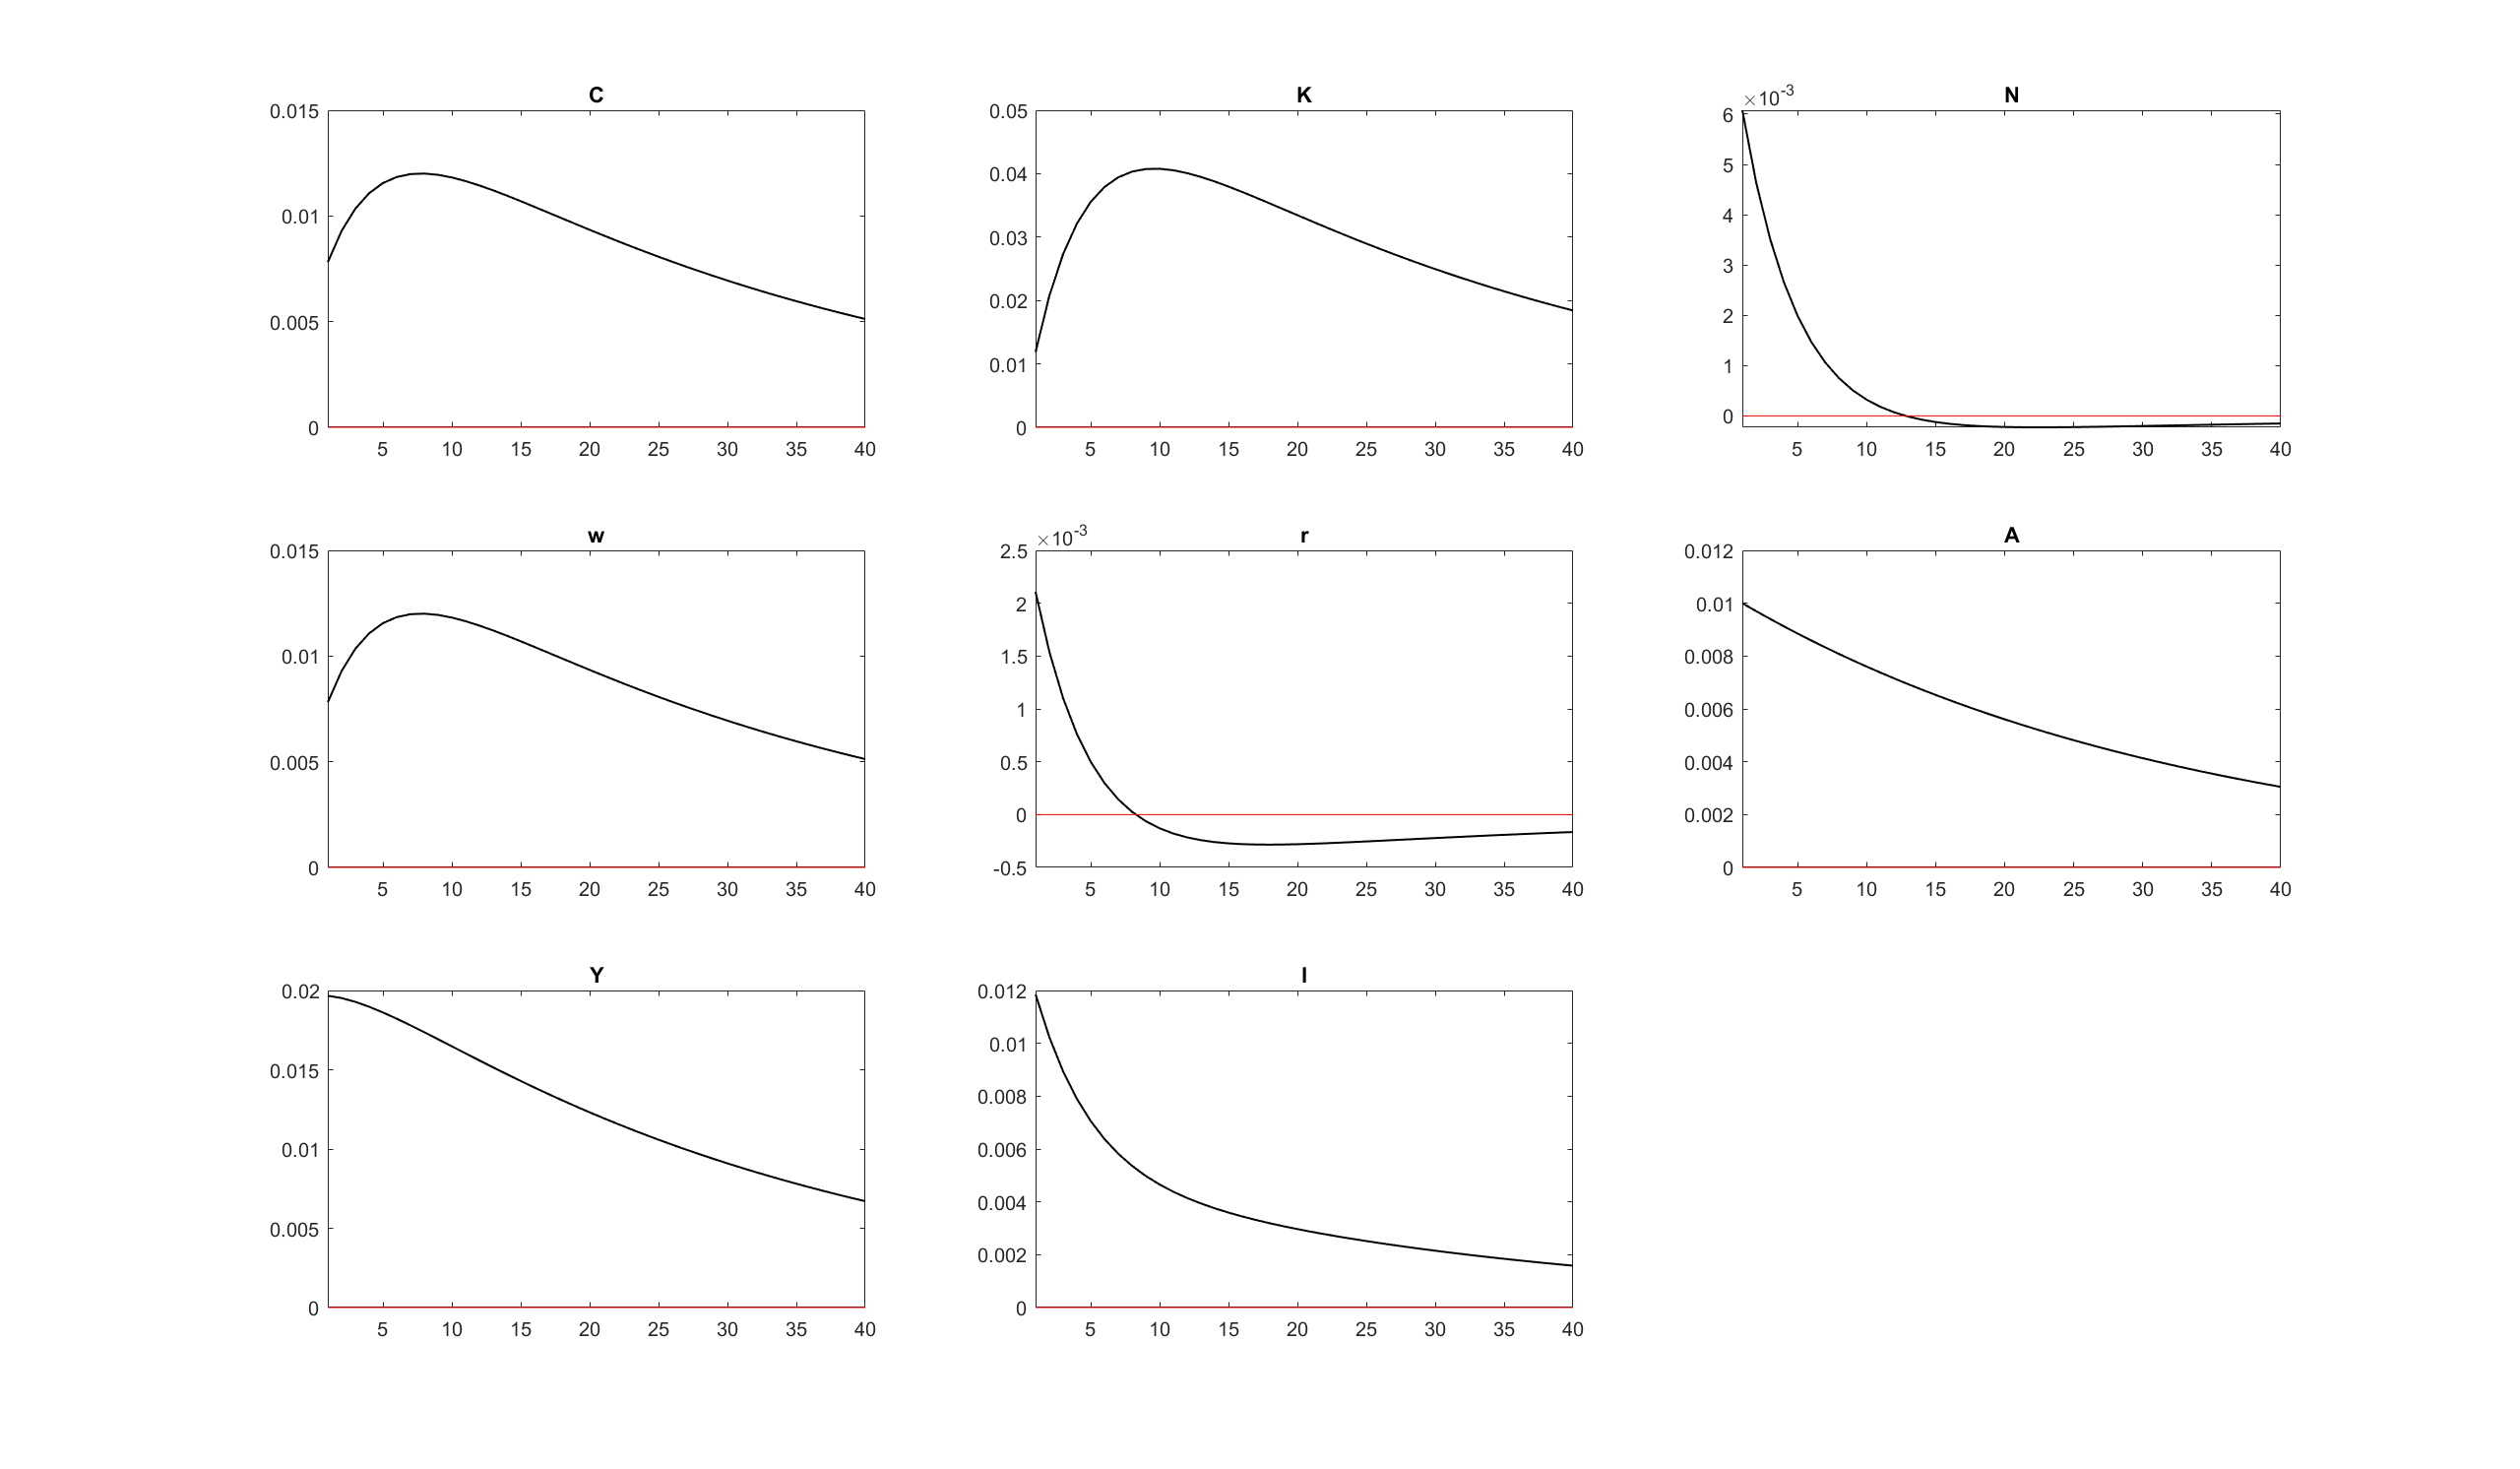
\includegraphics[width=1\textwidth]{figures/IRFs.png}
    \end{center}
    \caption{IRFs after productivity shock}
    \label{fig:graph}
\end{figure}

The shock is increase in TFP $A$ in the production function $A_{t}\left(\dfrac{k_{t-1}}{1+g}\right)^{\alpha}n^{1-\alpha}_{t}$. I add the economy's growth here.

Assume the process of productivity shock:

$\log\left(A_{t}\right)=\lambda A_{t-1}+e_{t}$

We also assume that $|\lambda|<1$ to make sure that there exists a steady state. The shock enters $e_{t}$ here.

As shown above, all the endogenous variables come into steady state gradually. 

Consumption, capital and wage go up for some time then come into a steady state. 

Labor, real interest rate converges to steady state quickly. 

The decreasing speed of TFP, output $Y$ and investment lies in between.

\subsubsection*{\textrm{e.}}

\begin{lstlisting}[basicstyle=\footnotesize\ttfamily]
    MATRIX OF CORRELATIONS (HP filter, lambda = 1600)
    Variables         C       K       N       w       r       A       Y       I
    C            1.0000  0.9247  0.5721  1.0000  0.4940  0.9212  0.9403  0.7775
    K            0.9247  1.0000  0.2167  0.9247  0.1257  0.7036  0.7399  0.4795
    N            0.5721  0.2167  1.0000  0.5721  0.9957  0.8462  0.8171  0.9606
    w            1.0000  0.9247  0.5721  1.0000  0.4940  0.9212  0.9403  0.7775
    r            0.4940  0.1257  0.9957  0.4940  1.0000  0.7934  0.7604  0.9308
    A            0.9212  0.7036  0.8462  0.9212  0.7934  1.0000  0.9986  0.9610
    Y            0.9403  0.7399  0.8171  0.9403  0.7604  0.9986  1.0000  0.9451
    I            0.7775  0.4795  0.9606  0.7775  0.9308  0.9610  0.9451  1.0000
\end{lstlisting}

We can see the correlations of endogenous in the output \texttt{Y} row or column.

The correlations w.r.t \texttt{C} and \texttt{I} are higher than the data, but in the same direction.

\texttt{N} is pretty close to the data.

\subsubsection*{\textrm{f.}}

\begin{lstlisting}
    THEORETICAL MOMENTS (HP filter, lambda = 1600)
    VARIABLE         MEAN  STD. DEV.   VARIANCE
    C              1.0030     0.0137     0.0002
    K              3.1253     0.0404     0.0016
    N              0.9065     0.0073     0.0001
    w              1.0030     0.0137     0.0002
    r              0.1455     0.0026     0.0000
    A              1.0000     0.0130     0.0002
    Y              1.3571     0.0263     0.0007
    I              0.3541     0.0142     0.0002
\end{lstlisting}

From the result we construct:

\begin{lstlisting}
    col1=[0.0137, 0.0404, 0.0073, 0.0137, 0.0026, 0.0130, 0.0263, 0.0142]
    col2=[0.0263, 0.0263, 0.0263, 0.0263, 0.0263, 0.0263, 0.0263, 0.0263]
    col3=col1./col2
col3 =

    0.5209    1.5361    0.2776    0.5209    0.0989    0.4943    1.0000    0.5399
\end{lstlisting}

To be more precise:

\begin{lstlisting}
    S=sqrt(oo_.var)
    T=S(7:7)
    D=diag(S/T)
D = 
    0.5195
    1.5361
    0.2771
    0.5195
    0.0978
    0.4957
    1.0000
    0.5412
\end{lstlisting}

The relative average volatility of \texttt{C}, \texttt{K}, \texttt{N}, \texttt{w}, \texttt{r}, \texttt{A}, \texttt{Y}, \texttt{I}, respectively, relative to output \texttt{Y}.

\texttt{C} \& \texttt{N} varies a little bit less than data, but still less than the variation in \texttt{Y}.

\texttt{I} varies less in the model, but in the data, investment varies more than output.

\subsubsection*{\textrm{g.}}

Though the directions of some variables match the data, it falls short in the prediction of the degree of investment change. Moreover, it doesn't take the sticky prices into account. 

\section*{\textbf{Appendix}}

Substituting equation (5) into (2) we have:

$\dfrac{U_{l}\left(c_{t},1-n_{t}\right)}{W_{t}}=-\beta\left(\lambda_{t+1}+\mu_{t+1}\right)$

$\because\mu_{t}=i_{t}\lambda_{t}$

$\therefore \dfrac{U_{l}\left(c_{t},1-n_{t}\right)}{W_{t}}=-\beta\left(\lambda_{t+1}+i_{t+1}\lambda_{t+1}\right)=-\beta\left(1+i_{t+1}\right)\lambda_{t+1}$

Because from (2) we have:

$\dfrac{U_{l}\left(c_{t+1},1-n_{t+1}\right)}{W_{t+1}}=-\lambda_{t+1}$

$\therefore \dfrac{U_{l}\left(c_{t},1-n_{t}\right)}{W_{t}}=\beta\left(1+i_{t+1}\right)\cdot\dfrac{U_{l}\left(c_{t+1},1-n_{t+1}\right)}{W_{t+1}}$

$\iff$

$\dfrac{U_{l}\left(c_{t},1-n_{t}\right)}{U_{l}\left(c_{t+1},1-n_{t+1}\right)}=\beta\left(1+i_{t+1}\right)\cdot\dfrac{W_{t}}{W_{t+1}}$

$\iff$

$\dfrac{U_{l}\left(c_{t},1-n_{t}\right)}{U_{l}\left(c_{t+1},1-n_{t+1}\right)}\cdot\dfrac{W_{t+1}}{W_{t}}=\beta\left(1+i_{t+1}\right)$

By Fisher Equation,

$1+i_{t+1}=\left(1+\pi_{t+2}\right)\left(1+r_{t+1}\right)=\dfrac{P_{t+2}}{P_{t+1}}\left(1+r_{t+1}\right)$

$\therefore\dfrac{U_{l}\left(c_{t},1-n_{t}\right)}{U_{l}\left(c_{t+1},1-n_{t+1}\right)}\cdot\dfrac{W_{t+1}}{W_{t}}=\beta\cdot\dfrac{P_{t+2}}{P_{t+1}}\left(1+r_{t+1}\right)$

$\therefore\dfrac{U_{l}\left(c_{t},1-n_{t}\right)}{U_{l}\left(c_{t+1},1-n_{t+1}\right)}\cdot\dfrac{W_{t+1}}{W_{t}}\cdot\dfrac{P_{t+1}}{P_{t+2}}=\beta\left(1+r_{t+1}\right)$

$\dfrac{U_{l}\left(c_{t},1-n_{t}\right)}{U_{l}\left(c_{t+1},1-n_{t+1}\right)}\cdot\dfrac{w_{t+1}P_{t+1}}{w_{t}P_{t}}\cdot\dfrac{P_{t+1}}{P_{t+2}}=\beta\left(1+r_{t+1}\right)$

If $P_{t}P_{t+2}=P^{2}_{t+1}$,

$\dfrac{U_{l}\left(c_{t},1-n_{t}\right)}{U_{l}\left(c_{t+1},1-n_{t+1}\right)}\cdot\dfrac{w_{t+1}}{w_{t}}=\beta\left(1+r_{t+1}\right)$

By Fisher Equation,

$1+i_{t}=\left(1+\pi_{t+1}\right)\left(1+r_{t}\right)=\dfrac{P_{t+1}}{P_{t}}\left(1+r_{t}\right)$

$P_{t}\left(1+i_{t}\right)=P_{t+1}\left(1+r_{t}\right)$

$P_{t+1}=\dfrac{P_{t}\left(1+i_{t}\right)}{1+r_{t}}$

$1+i_{t+1}=\left(1+\pi_{t+2}\right)\left(1+r_{t+1}\right)=\dfrac{P_{t+2}}{P_{t+1}}\left(1+r_{t+1}\right)$

$\iff$

$1+r_{t+1}=\dfrac{P_{t+1}}{P_{t+2}}\left(1+i_{t+1}\right)=\dfrac{1+i_{t+1}}{P_{t+2}}P_{t+1}=\dfrac{1+i_{t+1}}{P_{t+2}}\cdot\dfrac{P_{t}\left(1+i_{t}\right)}{1+r_{t}}$

$\dfrac{U_{l}\left(c_{t},1-n_{t}\right)}{U_{l}\left(c_{t+1},1-n_{t+1}\right)}\cdot\dfrac{w_{t+1}P_{t+1}}{w_{t}P_{t}}\cdot\dfrac{P_{t+1}}{P_{t+2}}=\beta\left(\dfrac{1+i_{t+1}}{P_{t+2}}\cdot\dfrac{P_{t}\left(1+i_{t}\right)}{1+r_{t}}\right)$

$\iff$

$\dfrac{U_{l}\left(c_{t},1-n_{t}\right)}{U_{l}\left(c_{t+1},1-n_{t+1}\right)}\cdot\dfrac{w_{t+1}P_{t+1}}{w_{t}P_{t}}\cdot P_{t+1}=\beta\left(\left(1+i_{t+1}\right)\cdot\dfrac{P_{t}\left(1+i_{t}\right)}{1+r_{t}}\right)$

$\iff$

$\dfrac{U_{l}\left(c_{t},1-n_{t}\right)}{U_{l}\left(c_{t+1},1-n_{t+1}\right)}\cdot\dfrac{w_{t+1}P^{2}_{t+1}}{w_{t}P^{2}_{t}}=\dfrac{\beta\left(1+i_{t+1}\right)\left(1+i_{t}\right)}{1+r_{t}}$

$\iff$

$\dfrac{U_{l}\left(c_{t},1-n_{t}\right)}{U_{l}\left(c_{t+1},1-n_{t+1}\right)}\cdot\dfrac{w_{t+1}}{w_{t}}\left(1+\pi_{t+1}\right)^{2}=\dfrac{\beta\left(1+i_{t+1}\right)\left(1+i_{t}\right)}{1+r_{t}}$

\end{document}